\FloatBarrier
\section{Stage 5: Critical reflection}
\subsection{Identify the limiting tested decision}
\label{sec:r51}
For the declared 12-condition objective and original feasibility rules,
the limiting tested decision is retaining 14 bit in the existing
sequential natural-binary/Hamming layout. Increasing to 16 bit is the
only tested feasible change with a positive adjusted objective-gain
interval. Small quantisation power does not imply that this is simply
dominant quantisation noise; the experiment tests the complete chain.

R4's unchanged cohort diagnoses main-domain channel power
$\RfiveMainChannel $, Gaussian power $\RfiveMainGaussian $ and quantisation
power $\RfiveMainQuant $, retaining signed cross terms. This locates loss
but does not establish a causal design ranking. I therefore predeclare
nine one-decision variants: baseline; 385-tap half-width 60/80 Hz;
257/513 taps at 70 Hz; 16 bit; Hamming(15,11); repetition(5,1); no ECC.
Everything else retains the standard formulas, fixed matrices, original
signal, range and full-grid metric.

Twenty new study-5 pilot bundles plan 350 new confirmation bundles;
300 fails the frozen rule, 350 passes. Each bundle runs all nine variants
at 15 conditions: the 12 main conditions plus three zero-main-weight
diagnostics ($p=0.3,0.5$ at the anchor SNR, and 40 dB at the personal $p$).
Thus $350\times9\times15=47\,250$ confirmation paths are run;
only the 12 main conditions enter the objective. Eq.~\eqref{eq:r51-planning}
uses tolerance $\max(0.01,0.05|\bar g_{\rm pilot}|)$; actual confirmation
half-widths meet all frozen targets. The approximate 19-statistic family
contains eight main gains, eight personal gains and three personal
means for R5.2. Gains use Eq.~\eqref{eq:r51-gain}; whole bundles are
the independent units. R4 and pilot records do not enter these means.
Same layouts share masks within a bundle; changed lengths use separate
registered layouts. Alternative-method replay (Section~\ref{sec:r61})
checks all confirmation paths within MSE
$\RfiveIndependentMse$; kernels also pass cosine-sum checks.

\begin{table}[htbp]
 \centering\small
 \caption{New R5 confirmation: objective and paired gains from 350 bundles, approximate 19-family intervals. Feasibility means original 1 \% gain/twofold expansion rules; absolute rates remain visible.}
 \label{tab:r51-decisions}
 \begin{tabular}{llrrr}
\toprule
One change & Feasible & kbit/s & Mean $J$ & Paired $J$ reduction [interval] \\
\midrule
Half-width 60 Hz & No & 392.00 & 2.58890 & $1.4624\times10^{-3}\ [1.3297\times10^{-3},1.5952\times10^{-3}]$ \\
Half-width 80 Hz & No & 392.00 & 2.59431 & $-3.9526\times10^{-3}\ [-4.0412\times10^{-3},-3.8640\times10^{-3}]$ \\
257 taps & No & 392.00 & 2.61074 & $-2.0373\times10^{-2}\ [-2.0651\times10^{-2},-2.0096\times10^{-2}]$ \\
513 taps & Yes & 392.00 & 2.59185 & $-1.4839\times10^{-3}\ [-1.5551\times10^{-3},-1.4127\times10^{-3}]$ \\
16 bit & Yes & 448.00 & 2.42149 & $1.6887\times10^{-1}\ [1.5944\times10^{-1},1.7830\times10^{-1}]$ \\
Hamming(15,11) & Yes & 305.46 & 5.01125 & $-2.4209\times10^{0}\ [-2.4324\times10^{0},-2.4094\times10^{0}]$ \\
Repetition(5,1) & No & 1120.00 & 0.45581 & $2.1345\times10^{0}\ [2.1268\times10^{0},2.1423\times10^{0}]$ \\
Uncoded & Yes & 224.00 & 6.65212 & $-4.0618\times10^{0}\ [-4.0747\times10^{0},-4.0488\times10^{0}]$ \\
\bottomrule
\end{tabular}

 
 
\end{table}


\begin{figure}[htbp]
 \centering
 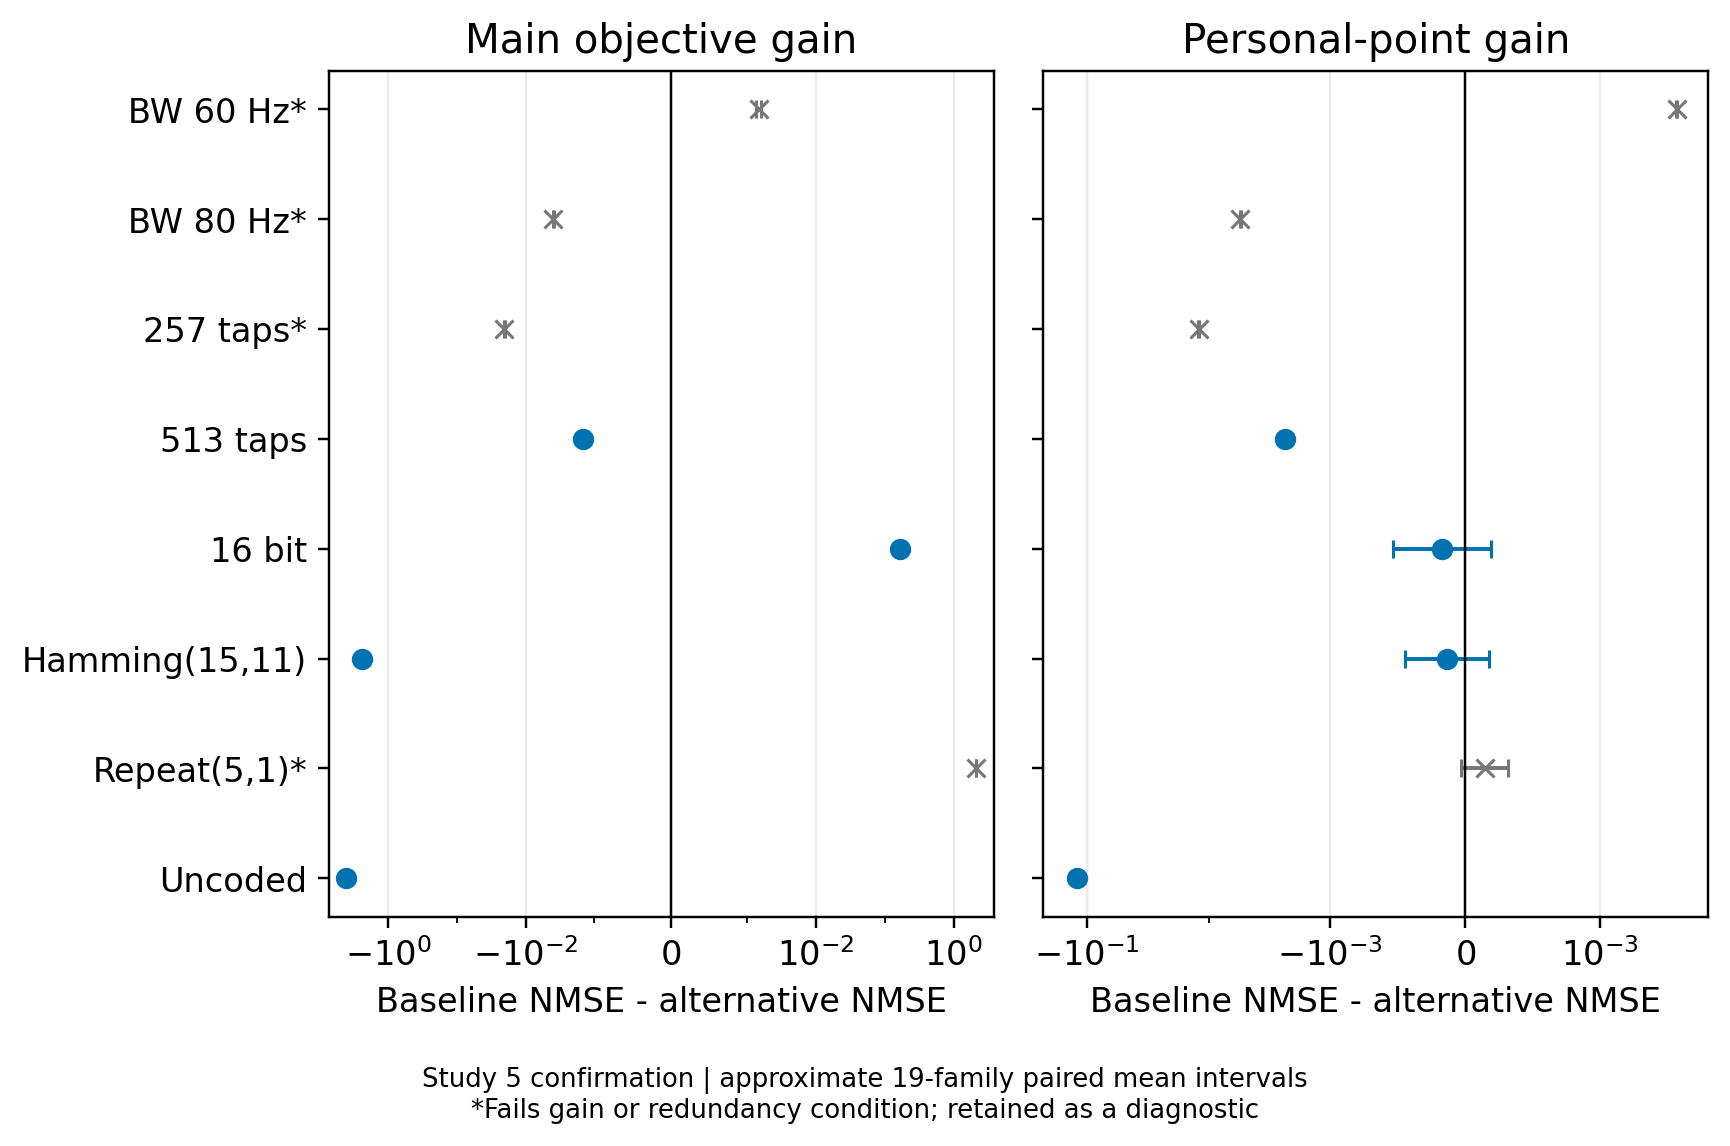
\includegraphics[width=.80\linewidth]{images/r51_counterfactual_gains.png}
 \caption{Single-decision gains with 19-family intervals. Grey crosses fail original feasibility rules; repetition cannot be a feasible winner. Symmetric-log panels retain negative/small effects and use distinct ranges.}
 \label{fig:r51-gains}
\end{figure}

\begin{samepage}
Baseline objective $\RfiveBaseJ $ falls with 16 bit by $\RfiveBitsGain $,
interval $[\RfiveBitsLower,\RfiveBitsUpper]$, at 392 $\to $448 kbit/s
(14.29 \% more traffic). Same-cohort prechannel improvement is only
$\RfiveBitsPreGain $. Most gain is in channel terms, not a 16-fold
total-error reduction predicted from $\Delta^2/12 $.
Eq.~\eqref{eq:r51-quant-ratio} gives the component ratio;
Eq.~\eqref{eq:r51-bit-coupling} retains joint decoded-bit interactions.
Fourteen-bit sample starts alternate at offsets 0/2 modulo 4; 16 bit starts
stay aligned. This diagnosis does not isolate alignment from every
other consequence of changing bit depth. The anchor-point gain
interval includes zero, so no personal improvement is established.
\end{samepage}

\FloatBarrier
\noindent\begin{minipage}{\linewidth}
\paragraph{Supplementary check: change packing only.}
Fix the clean input, 385-tap FIR, 14-bit labels, Hamming(7,4) and
392 kbit/s; Gaussian is absent. Compare sample-major packing with
MSB-first bit planes, applying the public inverse permutation after decoding.
All 128 BSC patterns per codeword give conditional expected full-grid NMSE
(Eq.~\eqref{eq:packing-expectation}, subject to numerical precision).
This supplementary diagnostic lies outside the nine-candidate selection
and 19-statistic family; only grouping changes, with expected BER fixed.
\end{minipage}\par

\begin{table}[H]
 \centering\small
 \caption{Fixed-14-bit packing: BSC-expected NMSE, Gaussian absent;
 both layouts send 392 kbit/s. Values are expectations, not confirmation
 means or confidence intervals.}
 \label{tab:r51-packing}
 \begin{tabular}{lrr}
\toprule
$p$ & Sample-major & Bit-plane \\
\midrule
0 & 0.000314845 & 0.000314845 \\
0.000210996 & 0.000485717 & 0.000551836 \\
0.01 & 0.372083 & 0.517315 \\
0.1 & 27.2268 & 36.9535 \\
\bottomrule
\end{tabular}

 
 
\end{table}

Results coincide at $p=0$; bit-plane expected NMSE is larger at all three
positive tested probabilities. Grouping therefore affects waveform error,
but this layout does not improve it or explain all of the 16-bit gain.
Block-outcome/SciPy reconstruction checks the moments; all 16 messages
and 128 patterns verify decoder translation invariance.
Figure~\ref{fig:r51-packing} is a shared-mask illustration, not a gain estimate.

\begin{figure}[H]
 \centering
 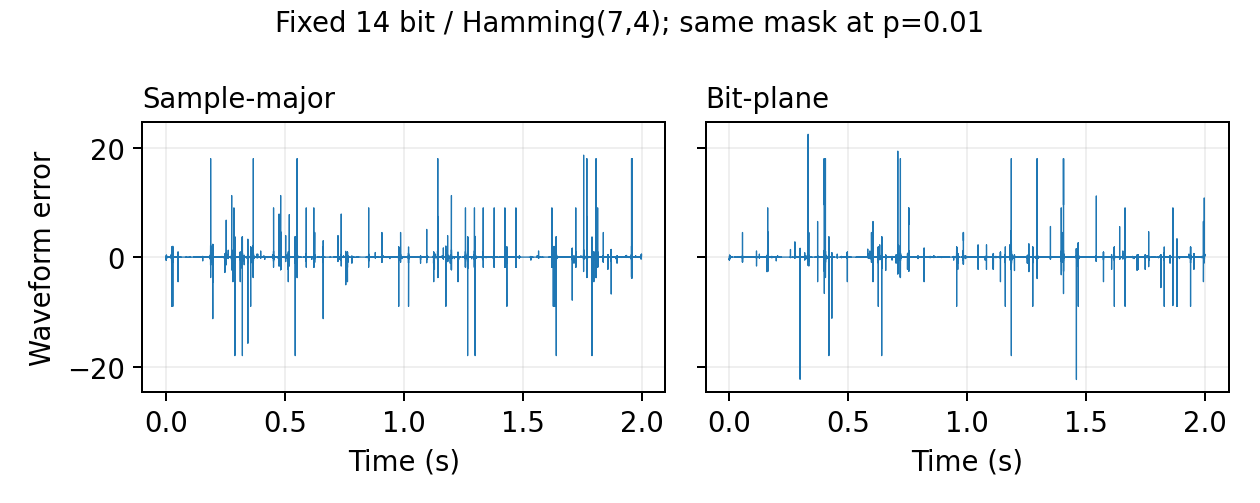
\includegraphics[width=.82\linewidth]{images/r51_packing_diagnostic.png}
 \caption{Same-mask waveform errors at $p=0.01$, Gaussian absent;
 quantiser, code, rate and axes fixed. One realisation illustrates packing,
 not expected gain.}
 \label{fig:r51-packing}
\end{figure}


Repetition gains $\RfiveRepeatGain $, interval
$[\RfiveRepeatLower,\RfiveRepeatUpper]$, but sends 1120 kbit/s and violates
the original twofold expansion rule. It cannot be a feasible winner.
Hamming(15,11) worsens the objective to $\RfiveCodeOtherJ $.
At $ p=0.1 $, exact block-failure laws give
$\RfiveQSeven/\RfiveQFifteen/\RfiveQRepeat $ for H74/H15/repetition
(Eq.~\eqref{eq:r51-block-failure}); both Hamming codes correct one
error, repetition two. Higher code rate is not stronger correction.
The 513-tap feasible filter worsens the objective and raises group delay
12 $\to $16 ms; other filter variants fail the original tone-gain guard.
No runtime penalty is inferred from their equal FFT length.

This scoped conclusion concerns nine variants and the chosen severity
weights, not a global optimum or real-world channel frequencies.
Gaussian error dominates personally; FIR distortion matters at 40 dB.
The R1--R4 baseline remains frozen; reflection does not retrospectively
substitute the 16 bit alternative into its validation.
